\documentclass[tikz,border=8pt]{standalone}
\usepackage{amsmath,amssymb}
\usetikzlibrary{arrows.meta,calc,decorations.markings,decorations.pathmorphing,patterns,shapes.geometric,positioning,shadings,plotmarks}

\begin{document}
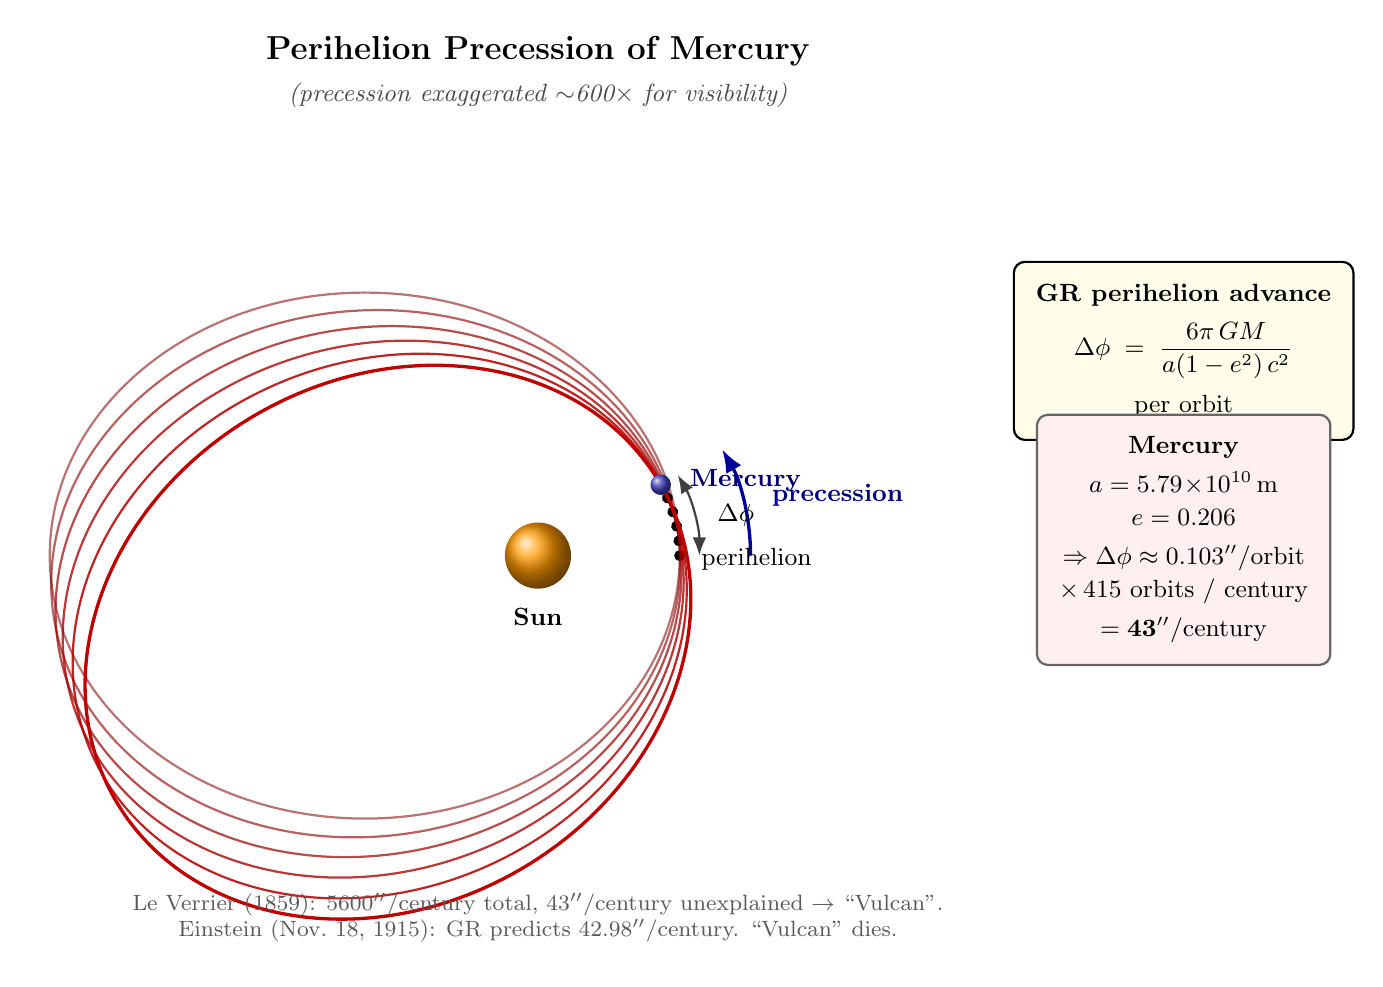
\begin{tikzpicture}[>=Latex]

  % --- Title ---------------------------------------------------------
  \node[font=\large\bfseries, align=center] at (0, 6.4) {%
    Perihelion Precession of Mercury};
  \node[font=\small\itshape, align=center, text=black!70] at (0, 5.85) {%
    (precession exaggerated $\sim$600$\times$ for visibility)};

  % --- Sun at center -------------------------------------------------
  \shade[ball color=orange!80!yellow] (0,0) circle (0.42);
  \node[font=\bfseries\small, anchor=north] at (0, -0.55) {Sun};

  % --- Parameters for ellipses ---------------------------------------
  % semi-major axis a = 4.0 cm (visual)
  % eccentricity e = 0.55 (visually nice; real Mercury 0.206 too round)
  % We rotate the axis by Delta phi each orbit. 5 orbits, total ~30 deg.
  % per-orbit step = 6 deg
  % Sun is at one focus; perihelion at angle = (axis angle) along +axis
  % focal distance c = a*e = 2.2 cm
  % perihelion radius r_p = a(1-e) = 1.8 cm

  % Orbit 1: axis at 0 deg
  % Orbit 2: axis at 6 deg
  % Orbit 3: axis at 12 deg
  % Orbit 4: axis at 18 deg
  % Orbit 5: axis at 24 deg
  % Orbit 6: axis at 30 deg

  % --- Draw the 6 ellipses (rotating around Sun = focus) -------------
  % An ellipse with Sun at focus: center is at distance c from Sun along +axis direction.
  % We use [rotate around={angle:(0,0)}] then shift the ellipse so its
  % +x-axis perihelion is at distance r_p = a-c from Sun.
  % Center of ellipse offset from Sun: -c along axis (focus is +c side).

  % Helper: \drawOrbit{angle}{color-intensity}
  % Use opacity scaling so newer orbits darker.

  % Orbit angles and styles (axis angles in degrees)
  % We'll draw with red-tone darkening.

  % Orbit at 0 deg
  \begin{scope}[rotate=0]
    \draw[thick, red!50!black, opacity=0.55] ([shift={(-2.2,0)}]0,0) ellipse (4.0 and 3.34);
    \fill[black] (1.8,0) circle (0.07);
  \end{scope}

  % Orbit at 6 deg
  \begin{scope}[rotate=6]
    \draw[thick, red!55!black, opacity=0.62] ([shift={(-2.2,0)}]0,0) ellipse (4.0 and 3.34);
    \fill[black] (1.8,0) circle (0.07);
  \end{scope}

  % Orbit at 12 deg
  \begin{scope}[rotate=12]
    \draw[thick, red!60!black, opacity=0.70] ([shift={(-2.2,0)}]0,0) ellipse (4.0 and 3.34);
    \fill[black] (1.8,0) circle (0.07);
  \end{scope}

  % Orbit at 18 deg
  \begin{scope}[rotate=18]
    \draw[thick, red!65!black, opacity=0.78] ([shift={(-2.2,0)}]0,0) ellipse (4.0 and 3.34);
    \fill[black] (1.8,0) circle (0.07);
  \end{scope}

  % Orbit at 24 deg
  \begin{scope}[rotate=24]
    \draw[thick, red!70!black, opacity=0.86] ([shift={(-2.2,0)}]0,0) ellipse (4.0 and 3.34);
    \fill[black] (1.8,0) circle (0.07);
  \end{scope}

  % Orbit at 30 deg (most recent)
  \begin{scope}[rotate=30]
    \draw[very thick, red!75!black, opacity=1.0] ([shift={(-2.2,0)}]0,0) ellipse (4.0 and 3.34);
    \fill[black] (1.8,0) circle (0.09);
    % Mercury planet on this orbit, at perihelion
    \shade[ball color=blue!50!gray] (1.8, 0) circle (0.13);
  \end{scope}

  % --- Mercury label (on outermost orbit's perihelion) ---------------
  \node[font=\small\bfseries, anchor=west, text=blue!40!black] at ({1.8*cos(30)+0.25}, {1.8*sin(30)+0.05}) {Mercury};

  % --- Perihelion label (first orbit) --------------------------------
  \node[font=\small, anchor=west] at (1.95, -0.05) {perihelion};

  % --- Precession arrow at outer arc ---------------------------------
  % Arrow showing rotation of major axis from 0 to 30 deg
  \draw[->, very thick, blue!60!black]
    (2.7, 0) arc[start angle=0, end angle=30, radius=2.7];
  \node[font=\small\bfseries, text=blue!50!black, anchor=west]
    at ({2.95*cos(15)}, {2.95*sin(15)}) {precession};

  % --- Delta phi label inside the arc --------------------------------
  \draw[<->, thick, black!75]
    (2.05, 0) arc[start angle=0, end angle=30, radius=2.05];
  \node[font=\small, text=black, anchor=west]
    at ({2.18*cos(15)+0.05}, {2.18*sin(15)-0.05}) {$\Delta\phi$};

  % --- Formula box (right side) --------------------------------------
  \node[draw=black, thick, rounded corners=4pt, fill=yellow!8,
        inner sep=8pt, align=center, font=\small] at (8.2, 2.6) {%
    \textbf{GR perihelion advance} \\[5pt]
    $\displaystyle \Delta\phi \;=\; \frac{6\pi\, GM}{a(1-e^{2})\, c^{2}}$ \\[5pt]
    per orbit};

  % --- Mercury number box -------------------------------------------
  \node[draw=black!60, thick, rounded corners=4pt, fill=red!6,
        inner sep=8pt, align=center, font=\small] at (8.2, 0.2) {%
    \textbf{Mercury} \\[3pt]
    $a=5.79\!\times\!10^{10}\,\mathrm{m}$ \\[1pt]
    $e=0.206$ \\[3pt]
    $\Rightarrow \Delta\phi \approx 0.103''/\mathrm{orbit}$ \\[1pt]
    $\times\, 415$ orbits $/$ century \\[3pt]
    $= \mathbf{43''/\mathrm{century}}$};

  % --- Historical note (bottom) -------------------------------------
  \node[font=\footnotesize, align=center, text=black!65] at (0, -4.6) {%
    Le Verrier (1859): $5600''/$century total, $43''/$century unexplained $\to$ ``Vulcan''.\\
    Einstein (Nov.\ 18, 1915): GR predicts $42.98''/$century. ``Vulcan'' dies.};

\end{tikzpicture}
\end{document}
